\documentclass[10pt,twocolumn,twoside,final]{IEEEtran}

% cite package, to clean up citations in the main text. Do not remove.
\usepackage{cite}
\usepackage{lastpage,fancyhdr,graphicx}
\usepackage{amssymb,amsmath}
\usepackage{mathtools}
\usepackage{hyperref}
\usepackage[square,sort,comma,numbers]{natbib}
\renewcommand{\bibfont}{\footnotesize}


% Remove brackets from numbering in List of References
\makeatletter
\renewcommand{\@biblabel}[1]{\quad#1.}
\makeatother

% *** SUBFIGURE PACKAGES ***
\ifCLASSOPTIONcompsoc
  \usepackage[caption=false,font=footnotesize,labelfont=sf,textfont=sf]{subfig}
\else
  \usepackage[caption=false,font=footnotesize]{subfig}
\fi

\begin{document}

\title{Proposal for Pediatric Health Centers in Uganda}


% author names and affiliations
% use a multiple column layout for up to three different
% affiliations
\author{\IEEEauthorblockN{Jonathan Lei,
Tafadar Soujad,
Ningyuan Zhang}\\
\IEEEauthorblockA{Cornell University, Ithaca, NY 14850 USA}
\thanks{Special thanks to Professor J. Varner (email:jdv27@cornell.edu).}}

\maketitle

\begin{abstract}
Pediatric health has been linked to the continued welfare of a population, and measures promoting it can lead to significant positive social outcomes, which is especially needed in third world countries like Uganda. While the methods of building and maintaining infrastructure related to pediatric health are well established, there lies a problem of such infrastructure requiring a significant amount of resources. We aim to build a fund that will properly address the necessary accumulation of the resources required for a pediatric health facility and 15 satellite clinics within a 100 mile radius of the city of Kampala, Uganda. This will be done with an endowment fund, the initial start up investment of which will be provided by the Bill and Melinda Gates Foundation. In doing so, this money will be put towards the purpose of building a self maintaining institution regarding pediatric health needs in and around Kampala, Uganda.
\end{abstract}


\section{Introduction}
Children's health is a significant concern in Uganda, resulting from various negative factors like HIV, malnutrition, lack of sanitation, vaccinations, insufficient drugs, and an insufficient number of motivated healthcare workers. Therefore, enhancements on local healthcare situation are meaningful to the local development and people’s life quality improvement.[1] 

On solving this task, we simulated the situation of establishing sustainable pediatric healthcare facilities in Uganda driven by a grant from the Bill and Melinda Gates Foundation, including a central medical facility and fifteen satellite clinics staffed with employees like doctors, physician assistants, facility managers and janitors. 

In this report, a robust financial strategy is introduced, which encompasses the project cost estimation, long-term investment strategy and post-project plan to ensure continuous operation. The investment portfolio is constructed and evaluated based on simulation results aligned with the historical risky asset pricing data. According to the simulation, the portfolio highly outperforms the SPY benchmark in actual data during our first year and the proposed investment strategy is theoretically able to ensure permanent operation on the constructed facilities.


\section{Results}

We observe in Figure 1 that not only will our planned investemnt portfolio provide necessary and sufficient resources for the building and maintenance of this operation with the initial funding of 95 Million USD from the Bill and Melinda Gates Foundation, but also for the continued funding and growth of our base endowment fund. We see here an expected positive trend for our investment portfolio, and for our overall operations. The initial gain is the actual gain of the portfolio so far in 2023, while the subsequent years' gains are calculated using an expected 10.5\% gain for our chosen portfolio to be reallocated. This initial trend culminates at the end of the first 10 year period, at which point the endowment is repaid, but by then enough capital gains have been reinvested that continued growth is possible, despite costs.

% Figures: Change me as needed. Figures do not need to be PDF format
\begin{figure}[!h]\centering
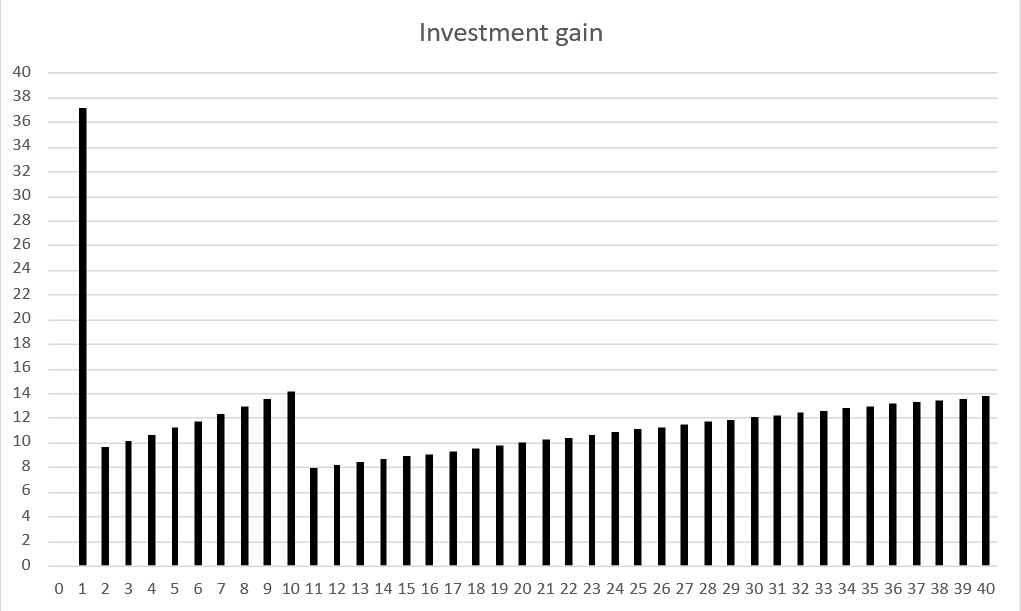
\includegraphics[width=0.47\textwidth]{./figs/60MIG.png}
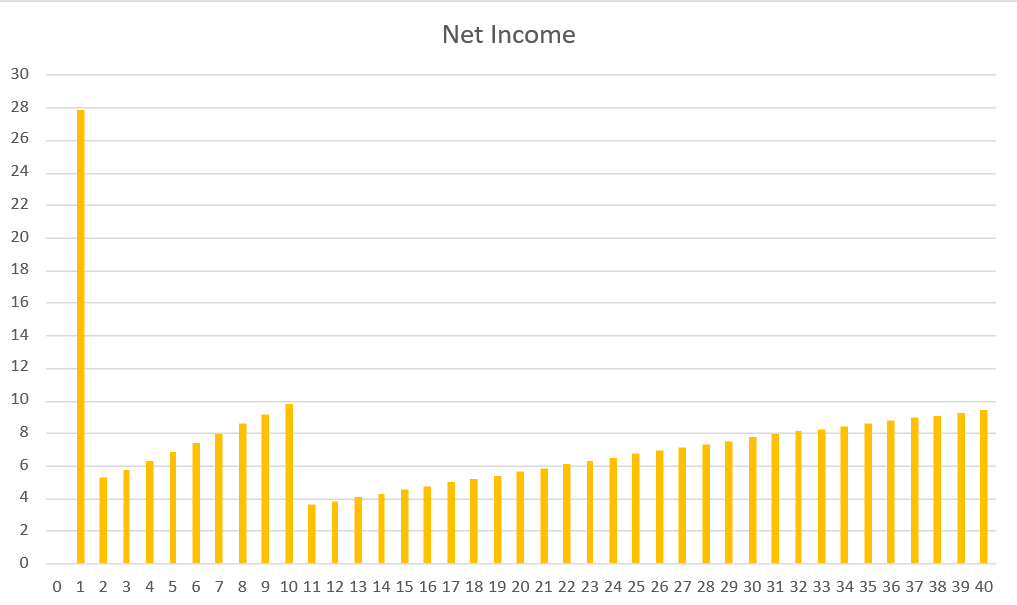
\includegraphics[width=0.47\textwidth]{./figs/60MNI.png}
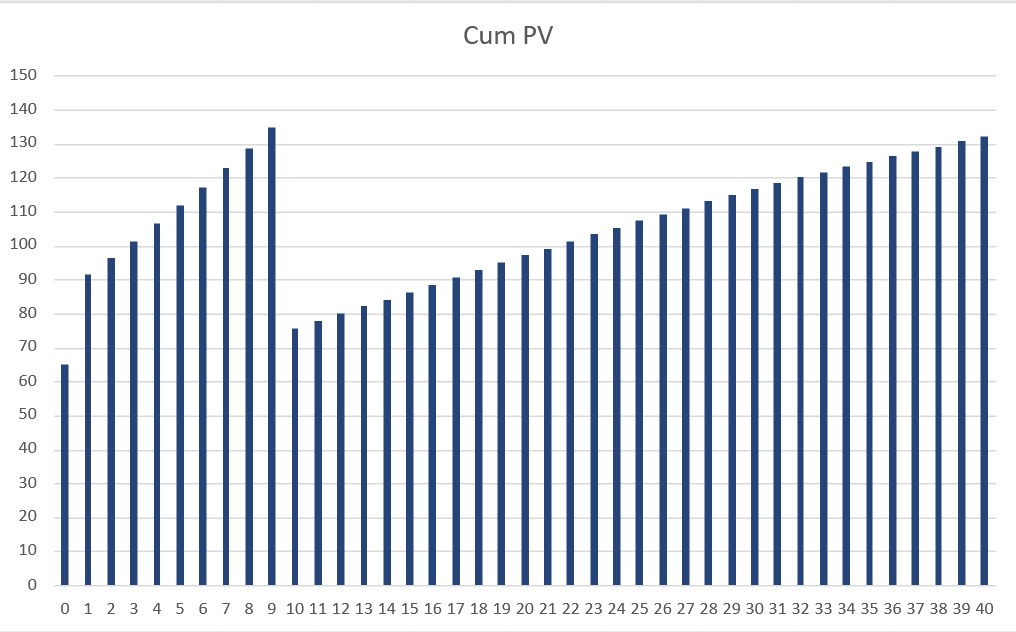
\includegraphics[width=0.47\textwidth]{./figs/60MNPV.png}
\caption{These graphs show the expected trends through time for the investment gain of our portfolio, eventually transferred to 30 Year Treasury Bonds after the initial 10 years, the Net Income over a period of the first 40 years of this operation which takes into account the costs of the operation, and the Net Present Value of our operation at every year over the next 40 years which shows consistent growth even when costs are factored in.}
\end{figure}

\begin{figure}[!h]\centering
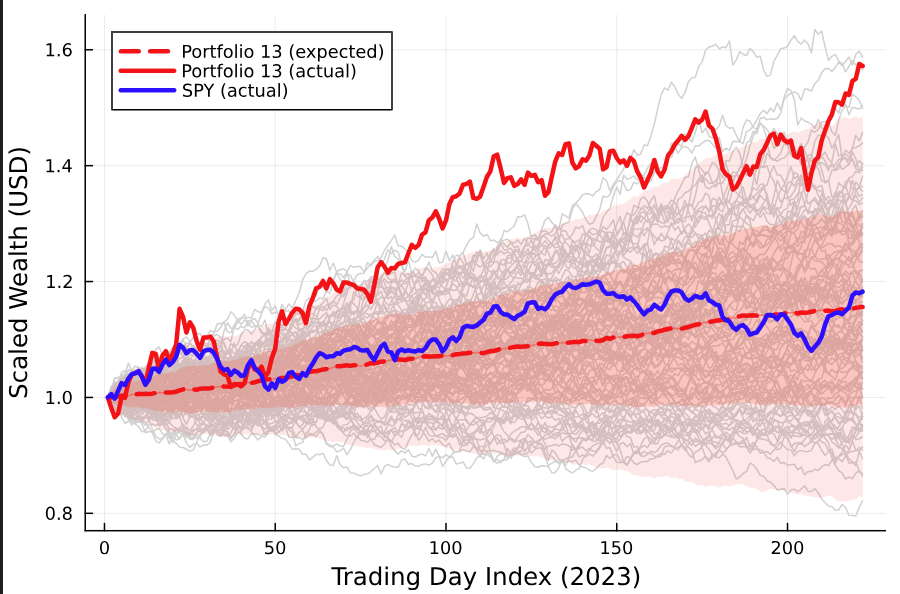
\includegraphics[width=0.5\textwidth]{./figs/year1expected.png}
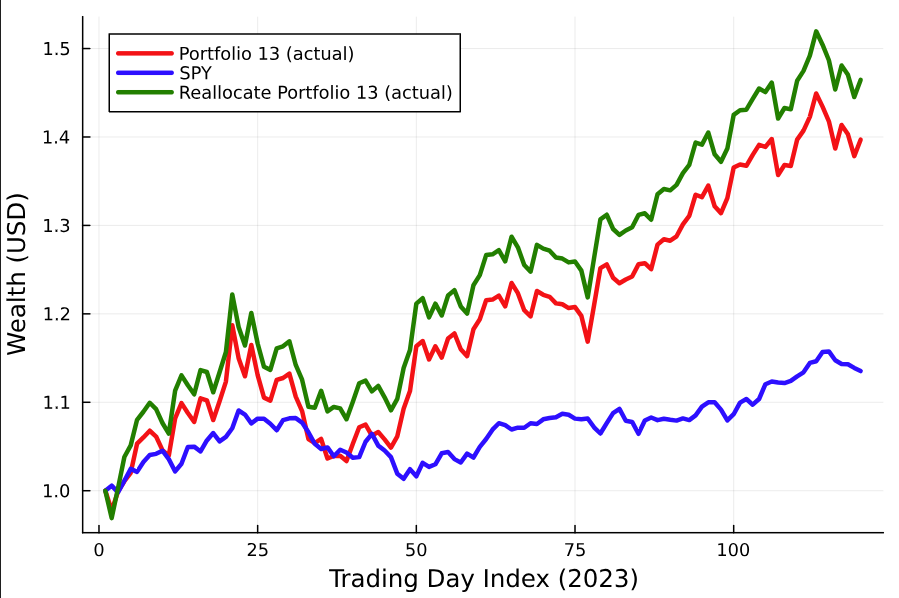
\includegraphics[width=0.5\textwidth]{./figs/year1reallocated.png}
\caption{We see that for the first year, our investment portfolio greatly exceeds our expectation and thus also our need. Dynamic reallocation is imbued into the portfolio among stocks of AMD, NVIDIA, Microsoft, Intel, Google, and Amazon. We also see from the top graph that this portfolio has an expected excess return of about 5.5\% or a total expected return of 10.5\%}
\end{figure}

\section{Discussion}
The discussion should be three paragraphs (or less). 
We see that our strategy provides an action plan for this operation. Th initial seed fund will provide the required funds to get the operation up and running, which we estimate to take about 1 year, after which we will assume normal operation. During the first 10 year period we will address the pediatric health needs of the local population while reinvesting any funds gained from our portfolio performance that was not used to cover the cost of operations into our portfolio. We designed this strategy so after 10 years, the funds provided by the Bill and Melinda Gates Foundation can be repaid in full. 

The reinvested funds are the pooled into 30 Year US Treasury bonds to provide a consistent return that will continue to cover the costs of operation. This 'risk-free' fund will also follow the same strategy of covering costs of operation and subsequent reinvestment, and is expected to still return a net positive growth in our available funds even after taking costs of operation into account. This can be repeated every 30 year term to provide perpetual funding for this operation. While it would be possible to keep pursuing an aggressive growth strategy for the fund in order to shield against any unforseen costs through a rigid stock portfolio such as the one we utilized for the initial 10 year period, we decided to rather go with the safer option of US Treasury Bonds as it already provides more than sufficient funding for operations and still maintains a growing body of funds.

There is however a concern for an exponentially growing costs. A long term project such as this that increases the well being of people by such a wide margin can have a positive social impact that results in the upwards development of a nation, which in turn would lead to staff needing to be paid more as time goes on as they would eventually no longer be paid salaries expected of workers in a third world country if our project helps Uganda develop and no longer be a third world country. We attempt to supplant the negative consequences of this possibility with a growing income even after the initial 10 year period.

\section{Materials and Methods}
We compiled a number of sources to determine the costs of building and maintaining this operation. The building and supplying of all infrastructure was understood to be an initial cost of 5 million USD. The cost of labor for doctors, physicians, secretaries, janitors, hospital administrator, medical malpractice insurance, and the operation of a central hospital, along with the operation of the clinics at the understood 10,000 USD a month totals to a yearly expense of just under 4.35 million USD.

For the operation of the portfolio, we chose various the stocks of various stable firms with histories of high performace. We implemented these stocks into a dynamic reallocation scenario, and accounted for the fact that we will pay back the face value of the seed fund generously provided to the Bill and Melinda Gates Foundation after a course of 10 years. Upon this, the remaining reinvested funds will be allocated towards into 30 year US Treasury Bonds which currently show an return interest rate of 4.750\% in order to provide a continuous 'risk free' source of funding for our operation. 

% This section should be here - update as needed
\section{Data and model availability}
The model equations were implemented in Julia and the needed resources were calculated with an amalgam of resources that were compiled in the Ugandan Endowment Data Microsoft Excel sheet.
The model code and Excel sheets are available at \url{https://github.com/trs-code/CHEME-5660-Ugandan-Endowment-Fund-Jonathan_L-Tafadar_S-Ningyuan_Z}

% References -
\bibliographystyle{naturemag_noURL}
\bibliography{Project}

\end{document}
\grid
